\documentclass[8pt]{beamer}
\usepackage{tikz}
\usepackage{tikz-cd}
\usepackage{qtree}
\usepackage{amsfonts}
\usepackage{amssymb}
\usepackage{amsmath}
\usepackage{amscd}
\usepackage{amsthm}
\usepackage{mathpartir}
\usepackage{bbm}
\usepackage[mathcal]{euscript}
\usepackage[utf8]{inputenc}
\setbeamertemplate{navigation symbols}{}%remove navigation symbols
%\usepackage[T1]{fontenc}
\usepackage{lmodern} \title{What is a scientific theory?}
\subtitle{or, how might you best formalize a scientific theory, were you inclined to do so?}
\author{Hans Halvorson and Jim Weatherall}
\date{September 8, 2013} \usetheme{Copenhagen}
\begin{document}
\def\2{\mathcal}
\def\7{\mathbb}
\newenvironment{proenv}{\only{\setbeamercolor{local structure}{fg=green}}}{}
\newenvironment{conenv}{\only{\setbeamercolor{local structure}{fg=red}}}{}  
\newenvironment{neuenv}{\only{\setbeamercolor{local
      structure}{fg=yellow}}}{}

%% A theory is _nothing less_ than a category ... but it may be more.


\begin{frame}

\maketitle


\end{frame}

\begin{frame}{Philosophy of science meets Hegel}

\textcolor{red}{\bf Syntactic view of theories:} A theory is a
  collection of \textcolor{red}{sentences} in a formal language.

\smallskip
\begin{itemize}
\item Carnap
\item Nagel
\end{itemize}

\bigskip \bigskip \textcolor{blue}{\bf The semantic revolution:} No,
scientific theories aren't like that.  A more accurate reconstruction
of a scientific theory will present it as a family of set-theoretic
structures.  \smallskip
\begin{itemize} 
\item Putnam: Theories cannot be syntactic things.
\item Suppes: A theory is a set-theoretic predicate.
\item van Fraassen: A theory is a collection of models.
\end{itemize}

\end{frame}

\begin{frame}{The semantic view of theories}

  {\Large \textbf{Slogan:} \newline \emph{A scientific theory should be
      identified with its class of models.}}

%% To Do: get quotes

\bigskip \textbf{\textcolor{red}{Innocuous?}}

\begin{itemize}
\item Jill North: Lagrangian and Hamiltonian mechanics are
  inequivalent, because their models are not isomorphic
\item To believe a theory is to believe that the WORLD is isomorphic
  to one of its models.
\end{itemize}


\bigskip \textbf{\textcolor{red}{Otiose?}}

\begin{itemize}
\item van Fraassen: Empiricism didn't work in the syntactic framework;
  it does work in the semantic framework.
\item John Bickle: Intertheoretic reduction didn't work in the
  syntactic framework; it does work in the semantic framework.
\end{itemize}

%% If it's innocuous, then it's otiose.  If not otiose, then wrong.

%% Are we asking the right questions?  van Fraassen said that the
%% syntactic view had led us to ask the wrong questions.  Are we now
%% making the same mistake again?  e.g. questions about
%% "representation" about "isomorphism".  Questions about equivalence
%% [North]




\end{frame}

\begin{frame}{Motivating example I}

\setlength{\tabcolsep}{3em}
\begin{table}
\centering
\begin{tabular}{lcccc} 
& Language & Axioms \\ \\ \hline \hline \\
$T_1$ & $\{ p_0,p_1,\dots \}$ & $\emptyset$ \\ \\ 
$T_2$ & $\{ p_0,p_1,\dots \}$ & $p_0\vdash p_i$ \end{tabular} 
\end{table}
\bigskip


%% TO DO: picture

\begin{figure}
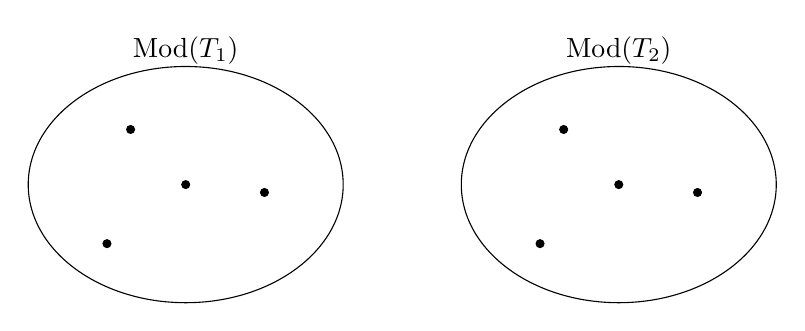
\begin{tikzpicture}
\draw (0,0) ellipse (2cm and 1.5cm);
\draw (5.5,0) ellipse (2cm and 1.5cm);

\node[align=center, below] at (0,2)%
{$\mathrm{Mod}(T_1)$};
\node[align=center, below] at (5.5,2)%
{$\mathrm{Mod}(T_2)$};

\node (A) at (0,0) {};
\draw[fill] (0,0) circle [radius=0.05];
\node (B) at (-0.7,0.7) {};
\draw[fill] (-0.7,0.7) circle [radius=0.05];
\node (C) at (1,-0.1) {};
\draw[fill] (1,-0.1) circle [radius=0.05];
\draw[fill] (-1,-0.75) circle [radius=0.05];

\node (X) at (5.5,0) {};
\draw[fill] (5.5,0) circle [radius=0.05];
\node (Y) at (4.8,0.7) {};
\draw[fill] (4.8,0.7) circle [radius=0.05];
\node (Z) at (6.5,-0.1) {};
\draw[fill] (6.5,-0.1) circle [radius=0.05];
\draw[fill] (4.5,-0.75) circle [radius=0.05];

\end{tikzpicture}
\end{figure}


\bigskip \textcolor{red}{Challenge:} How to distinguish
$\mathrm{Mod}(T_1)$ from $\mathrm{Mod}(T_2)$ when they are isomorphic
sets.






\end{frame}

\begin{frame}{Motivating example I}

%% [p_0] is isolated -- draw a picture
%% [p_0] is contained in all [p_i] -- draw a picture
%% TO DO: picture
\bigskip

\begin{figure}
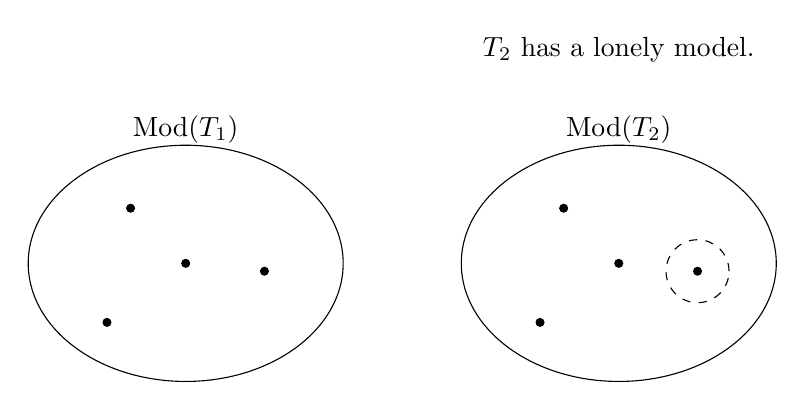
\begin{tikzpicture}
\draw (0,0) ellipse (2cm and 1.5cm);
\draw (5.5,0) ellipse (2cm and 1.5cm);

\node[align=center, below] at (0,2)%
{$\mathrm{Mod}(T_1)$};
\node[align=center, below] at (5.5,2)%
{$\mathrm{Mod}(T_2)$};
\node[align=center, below] at (5.5,3)%
{$T_2$ has a lonely model.};

\node (A) at (0,0) {};
\draw[fill] (0,0) circle [radius=0.05];
\node (B) at (-0.7,0.7) {};
\draw[fill] (-0.7,0.7) circle [radius=0.05];
\node (C) at (1,-0.1) {};
\draw[fill] (1,-0.1) circle [radius=0.05];

\draw[fill] (-1,-0.75) circle [radius=0.05];

\node (X) at (5.5,0) {};
\draw[fill] (5.5,0) circle [radius=0.05];
\node (Y) at (4.8,0.7) {};
\draw[fill] (4.8,0.7) circle [radius=0.05];
\node (Z) at (6.5,-0.1) {};
\draw[fill] (6.5,-0.1) circle [radius=0.05];
\draw[dashed] (6.5,-0.1) circle [radius=0.4];   %% make this dashed
\draw[fill] (4.5,-0.75) circle [radius=0.05];
\end{tikzpicture}
\end{figure}

\bigskip

\textcolor{purple}{Moral:} A theory doesn't just give us models, it
also gives us a notion of closeness of models.

\end{frame}



\begin{frame}{From a mathematical point of view}

\begin{description}
\item[Question:] Can a theory $T$ be reconstructed from
  $\mathrm{Mod}(T)\,$? \bigskip
\item[Clarification:] What kind of mathematical object is
  $\mathrm{Mod}(T)\,$? \bigskip
\item[Answer:] If $\mathrm{Mod}(T)$ is reduced to a bare set, then
  crucial information about $T$ has been lost.
 
  \bigskip Example: which theory has as its typical model $\{
  \emptyset ,\{ \emptyset \} ,\{ \{ \emptyset \} \} \}$?

%% Consider the class of groups
%% Consider the class of vector spaces over $\mathbb{R}$
%% Consider the  set {0,{0},{{0}}}

\bigskip
\item[Challenge:] Where does $\mathrm{Mod}(T)$ live in the
  mathematical universe?  What is the semantic content of a scientific
  theory?  \newline

\end{description}

\end{frame}




\begin{frame}{Stone duality theorem}

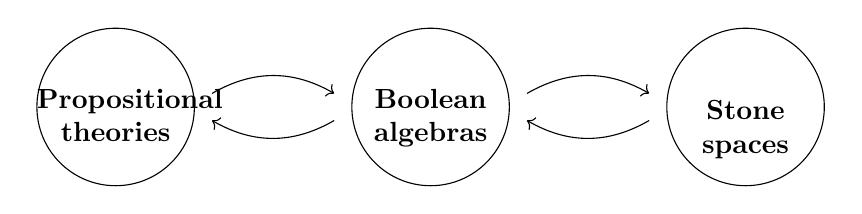
\begin{tikzpicture}
\draw (0,0) ellipse (1cm and 1cm);
\draw (4,0) ellipse (1cm and 1cm);
\draw (8,0) ellipse (1cm and 1cm);

\node (A) at (5.1,0.1) {};
\node (B) at (6.9,0.1) {};
\draw [->] (A) to [bend left=30] (B);
\node (C) at (5.1,-0.1) {};
\node (D) at (6.9,-0.1) {};
\draw [<-] (C) to [bend right=30] (D);

\node (E) at (1.1,0.1) {};
\node (F) at (2.9,0.1) {};
\draw [->] (E) to [bend left=30] (F);
\node (G) at (1.1,-0.1) {};
\node (H) at (2.9,-0.1) {};
\draw [<-] (G) to [bend right=30] (H);


\node[align=center, below,text width=2cm] at (0,0.35)%
{\textbf{Propositional theories}};
\node[align=center, below,text width=2cm] at (4,0.35)%
{\textbf{Boolean algebras}}; 
\node[align=center, below,text width=2cm] at (8,0.2)%
{\textbf{Stone spaces}};
\end{tikzpicture}

\bigskip $\mathrm{Mod}(T)$ is a topological space; and the Lindenbaum
algebra of $T$ can be recovered from its topological structure.


\bigskip \textcolor{purple}{Moral:} A theory doesn't just give us
models, it also gives us a notion of nearness of models.

\end{frame}






\begin{frame}{Motivating example II}

% \begin{table}
% \centering
% \begin{tabular}{lcccc} 
%   & & Language & & Axioms \\ \\ \hline \hline \\
%   $T_1$ & & $\emptyset$ & & $\exists _{=2}$ \\ \\ 
%   $T_2$ & & $\{ c\}$ & & $\exists _{=2}$ \end{tabular} 
% \end{table}

% \begin{itemize}
% \item If $|M|=|N|$ then there is an isomorphism $\sigma :M\to N$.
%   \newline $\Longrightarrow$ $T_1$ has a single model.

% \item If $|M|=|N|$ then there is an isomorphism $\sigma :M\to N$ such
%   that $\sigma (c^M)=c^N$.  \newline $\Longrightarrow$ $T_2$ has a
%   single model.
% \end{itemize}

\setlength{\tabcolsep}{3em}
\begin{table}
\centering
\begin{tabular}{lcccc}
& $T_1$ & $T_2$ \\ \\ \hline \hline \\
Language & $\emptyset$ & $\{ c\}$ \\ \\
Axioms & $\exists _{=2}$ & $\exists _{=2}$ \end{tabular}
\end{table}
\bigskip

\begin{figure}
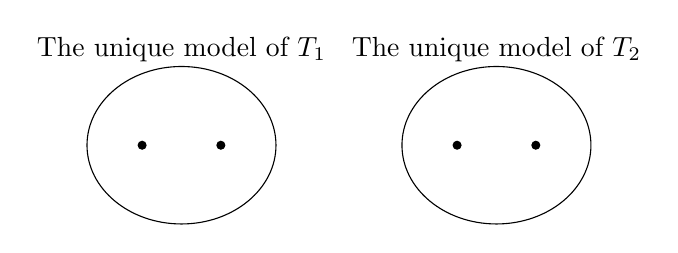
\begin{tikzpicture}
\draw (0,0) ellipse (1.2cm and 1cm);
\draw (4,0) ellipse (1.2cm and 1cm);

\node[align=center, below] at (0,1.5)%
{The unique model of $T_1$}; 
\node[align=center, below] at (4,1.5)%
{The unique model of $T_2$};
\draw[fill] (-0.5,0) circle [radius=0.05];
\draw[fill] (0.5,0) circle [radius=0.05];
\draw[fill] (3.5,0) circle [radius=0.05];
\draw[fill] (4.5,0) circle [radius=0.05];
\end{tikzpicture}
\end{figure}


\bigskip \textcolor{red}{Challenge:} How to distinguish
$\mathrm{Mod}(T_1)$ from $\mathrm{Mod}(T_2)$ when each consists of a
single isomorphism class?
\end{frame}



\begin{frame}{Motivating example II}

\begin{figure}
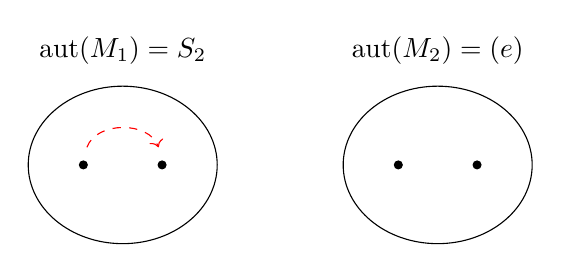
\begin{tikzpicture}
\node[align=center, below] at (0,1.75)%
{$\mathrm{aut}(M_1)=S_2$}; 
\node[align=center, below] at (4,1.75)%
{$\mathrm{aut}(M_2)=(e)$};

\draw (0,0) ellipse (1.2cm and 1cm);
\draw (4,0) ellipse (1.2cm and 1cm);

\node (A) at (-0.5,0.1) {};
\draw[fill] (-0.5,0) circle [radius=0.05];
\node (B) at (0.5,0.1) {};
\draw[fill] (0.5,0) circle [radius=0.05];
\draw [->,color=red,dashed] (A) to [bend left=70] (B);

\draw[fill] (3.5,0) circle [radius=0.05];
\draw[fill] (4.5,0) circle [radius=0.05];
\end{tikzpicture}
\end{figure}


\bigskip \textcolor{purple}{Moral:} A theory doesn't just give us
models, it also gives us arrows between models.

\end{frame}

\begin{frame}{What do equivalent theories share in common?}

%% de Bouvere

  \textbf{Standard Account:} $T_1$ and $T_2$ are
  \textcolor{red}{theoretically equivalent} just in case they have a
  common definitional extension.  (Glymour 1970, ``Theoretical realism
  and theoretical equivalence'')

  \bigskip \textbf{Fact:} $T'$ is a definitional extension of $T$ just
  in case the forgetful functor $G:\mathrm{Mod}(T')\to\mathrm{Mod}(T)$
  is:
\begin{itemize}
\item \textcolor{red}{essentially surjective:} each model of $T$ can be expanded to a
  model of $T'$.
\item \textcolor{red}{full:} each morphism between $T$ models is also a morphism
  between $T'$ models.
\item \textcolor{red}{faithful:} automatic since $G$ is the identity on arrows
\item \textcolor{red}{continuous in the logical topology:} automatic
\end{itemize}
\end{frame}


\begin{frame}{What do equivalent theories share in common?}

  \textbf{Corollary:} If $T$ and $T'$ are theoretically equivalent (in
  Glymour's sense), then $\mathrm{Mod}(T)$ and $\mathrm{Mod}(T')$ are
  isomorphic qua topological groupoids.


\end{frame}



\begin{frame}{Awodey-Forssell duality theorem}

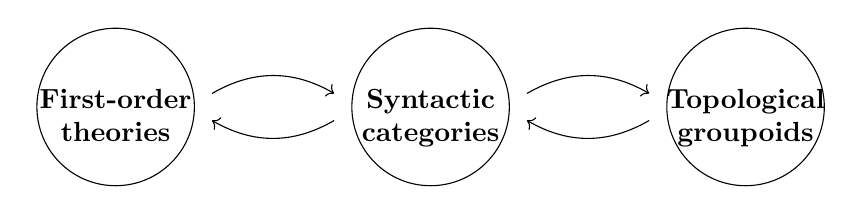
\begin{tikzpicture}
\draw (0,0) ellipse (1cm and 1cm);
\draw (4,0) ellipse (1cm and 1cm);
\draw (8,0) ellipse (1cm and 1cm);

\node (A) at (5.1,0.1) {};
\node (B) at (6.9,0.1) {};
\draw [->] (A) to [bend left=30] (B);
\node (C) at (5.1,-0.1) {};
\node (D) at (6.9,-0.1) {};
\draw [<-] (C) to [bend right=30] (D);

\node (E) at (1.1,0.1) {};
\node (F) at (2.9,0.1) {};
\draw [->] (E) to [bend left=30] (F);
\node (G) at (1.1,-0.1) {};
\node (H) at (2.9,-0.1) {};
\draw [<-] (G) to [bend right=30] (H);


\node[align=center, below,text width=2cm] at (0,0.35)%
{\textbf{First-order theories}};
\node[align=center, below,text width=2cm] at (4,0.35)%
{\textbf{Syntactic categories}}; 
\node[align=center, below,text width=2cm] at (8,0.35)%
{\textbf{Topological groupoids}};
\end{tikzpicture}

\bigskip $\mathrm{Mod}(T)$ is a topological groupoid; and the
syntactic category of $T$ can be recovered from its topological
groupoid structure.


\bigskip \textcolor{purple}{Moral:} The semantic content of a theory
includes relations between models, such as closeness of models and
arrows between models.

\end{frame}



\begin{frame}{Major morals}

  \begin{enumerate} \addtolength{\itemsep}{\baselineskip}
%   \item A theory doesn't just give us models, it also gives us
%     relations between models.
%   \item To compare two theories, we must compare their models
%     \emph{and} the relations between their models.
% \begin{itemize}
% \item Two theories could have the same models, but still be
%   inequivalent.  (Gauge theories)
% \item Believing a theory cannot amount to believing that the WORLD is
%   isomorphic to one of its models.
% \end{itemize}
\item Syntactic and semantic notions are \emph{dual} to each other.
  \begin{itemize}
  \item No important philosophical claim turns on viewing theories
    semantically instead of syntactically.
\end{itemize}
\item The syntactic category of a theory is a hybrid
  semantic-syntactic object.
\item Language-dependency is not peculiar to a syntactic account; in
  all cases, we need a notion of equivalence of theories.
\end{enumerate}
\end{frame}




\begin{frame}{Complications and questions}

\begin{itemize} 
\item Why just isomorphisms?  Why not all arrows?
\smallskip
\begin{itemize}
%% two theories: a b, c -> d 
\item Explanation via relations between models.
\end{itemize}
\bigskip
\item Which topology?  
\smallskip
\begin{itemize} 
\item For theories with a finite language, the logical topology is
  trivial.
\item What has the logical topology to do with other notions of
  similarity between models?
\end{itemize}
\bigskip
\item Relations between theories
%% explicated via kinds of functors
%% limiting relations between theories
\end{itemize}


\end{frame}



\begin{frame}{Repeating the mistakes of the past?}

\begin{itemize}
\item The syntactic view accused of giving rise to fruitless internal
  questions.  (see van Fraassen)
\item The semantic view gives rise to questions about
  ``representation'' that are of no concern in scientific practice
%% But categories are living mathematics
%% Bourbaki is dead
\end{itemize}
\end{frame}


%% Categories and topos cut mathematical reality at the joints.  The
%% notions of "full functors," "faithful functors," etc..

%% Morita equivalence -- relation to de Bouvere

%% Want to understand: why do we need only isomorphisms?  Why not
%% other arrows between the models?

%% What theoretical role is played by this additional structure,
%% i.e. isomorphisms and topology?


%% Transcending the semantic-syntactic dichotomy
%% syntactic presentation of a theory --> syntactic category <-->
%% semantic category <-- semantic presentation of a theory

%% Aufhebung

\end{document}




\end{description}
\begin{description}
\item[\begin{description}
\item[Fact:] 
